% Section III -- Architecture (target 380 words) + Fig. 1 (TikZ).
% Spec of record: v2/docs/ARCH_SPEC.md (frozen), v2/docs/FORMATS.md, DECISIONS D1/D2/D8/D13.
\section{Architecture}\label{sec:arch}
% Fig. 1 -- accelerator block diagram (TikZ, single column). Structure per v2/docs/ARCH_SPEC.md.
\begin{figure}[t]
\centering
\resizebox{\columnwidth}{!}{%
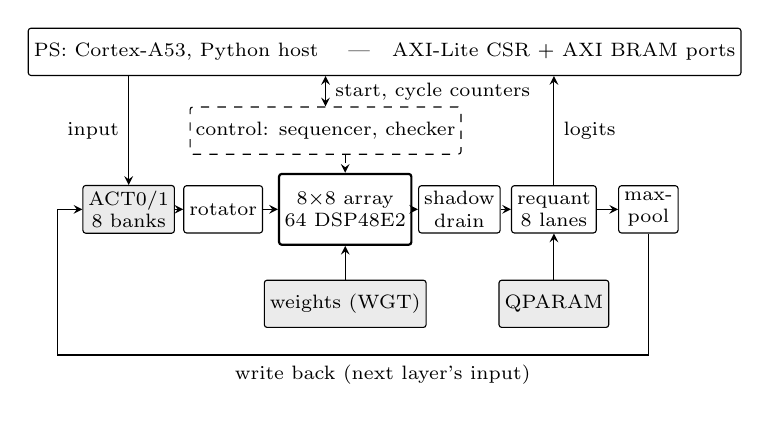
\begin{tikzpicture}[font=\scriptsize, >=stealth,
  blk/.style={draw, rounded corners=1pt, align=center, inner sep=2pt, minimum height=6mm},
  mem/.style={blk, fill=black!8},
  ctl/.style={blk, dashed}]
  % PS
  \node[blk, minimum width=7.9cm] (ps) at (-0.3,2.75)
      {PS: Cortex-A53, Python host \quad|\quad AXI-Lite CSR + AXI BRAM ports};
  % datapath (one row, left to right)
  \node[mem] (act)  at (-3.55,0.75) {ACT0/1\\8 banks};
  \node[blk] (rot)  at (-2.35,0.75) {rotator};
  \node[blk, line width=0.8pt, minimum height=9mm] (arr) at (-0.8,0.75) {$8{\times}8$ array\\64 DSP48E2};
  \node[blk] (drn)  at (0.65,0.75) {shadow\\drain};
  \node[blk] (rq)   at (1.85,0.75) {requant\\8 lanes};
  \node[blk] (pool) at (3.05,0.75) {max-\\pool};
  % memories and control (second row)
  \node[mem] (wgt) at (-0.8,-0.45) {weights (WGT)};
  \node[mem] (qp)  at (1.85,-0.45) {QPARAM};
  \node[ctl] (seq) at (-1.05,1.75) {control: sequencer, checker};
  % data flow
  \draw[->] (act) -- (rot);
  \draw[->] (rot) -- (arr);
  \draw[->] (arr) -- (drn);
  \draw[->] (drn) -- (rq);
  \draw[->] (rq) -- (pool);
  \draw[->] (wgt) -- (arr);
  \draw[->] (qp) -- (rq);
  \draw[->] (pool.south) -- (3.05,-1.1) -- (-4.45,-1.1) node[pos=0.45, below] {write back (next layer's input)} -- (-4.45,0.75) -- (act.west);
  \draw[dashed,->] (seq.south -| arr.north) -- (arr.north);
  % host interface
  \draw[->] (act.north |- ps.south) -- (act.north) node[pos=0.5, left] {input};
  \draw[<->] (seq.north |- ps.south) -- (seq.north) node[midway, right] {start, cycle counters};
  \draw[->] (rq.north) -- (rq.north |- ps.south) node[midway, right] {logits};
\end{tikzpicture}}
\caption{Accelerator organization. Weights and activations stay in BRAM; the host writes the input,
starts a job and reads the logits and cycle counters.}
\label{fig:arch}
\end{figure}


\textbf{Numeric contract.} Activations and weights are signed INT8 with
zero-point 0, a per-tensor activation scale and per-output-channel weight
scales; products accumulate in INT32. Each output channel stores
$(q_b, m, s)$: $v = \mathit{acc} + q_b$ is multiplied by the unsigned 32-bit
$m$, shifted right by $s$ with round-half-to-even, then passed through ReLU
and clipped to INT8. % src: ARCH_SPEC.md "Hardware requant"; B = 32 (DECISIONS D1 outcome)
The final layer exports raw INT32 logits, and the host applies the
reference's float32 dequantization and argmax.

\textbf{Datapath.} The core is an $8{\times}8$ output-stationary array of
DSP48E2 slices (Fig.~\ref{fig:arch}). Rows hold 8 consecutive output pixels
of one row and columns hold 8 output channels. Every cycle the array
consumes one reduction index $k = (ic, k_y, k_x)$: 8 activations and 8
weights are broadcast without skew, and the first product of a tile
overwrites the accumulator, so no clear cycle is needed. At the end of a
tile the 64 accumulators move to shadow registers, which drain one output
channel per cycle while the next tile accumulates. Eight requantization
lanes and a fused, bypassable $2{\times}2$ max-pool follow.
% src: ARCH_SPEC.md Datapath

\textbf{Memory.} Nothing leaves the chip during inference. Two ping-pong
activation buffers of 8 byte-wide banks hold a layer's input and output; a
pixel at column $x$ lives in bank $x \bmod 8$. For kernel offset $k_x$,
bank $b$ supplies output row $(b - k_x) \bmod 8$ and a byte rotator restores
the order, so all 8 operands arrive in one cycle without conflicts. All
weights stay resident in a 64-bit-wide weight memory.
% src: ARCH_SPEC.md Memory

\textbf{Control and interface.} Addresses come from counters and additions
only; the host precomputes derived fields in a 16-word descriptor per layer.
Data and control travel together as tokens through the pipeline, so no
stage infers timing by counting cycles. A sequencer runs up to 8 layers per
start, and a pipelined checker refuses illegal descriptors with an error
code before any work starts. % src: ARCH_SPEC.md Controller; DECISIONS D8-1, D13
The PS sees an AXI-Lite register file with 64-bit total-cycle, MAC-active
and stall counters, per-layer cycle counters, 16 logit registers and a
BUILD\_ID; the design loads as a PYNQ overlay. % src: ARCH_SPEC.md CSR
Of its 16,538 LUTs, the core uses 3,338; the rest is the AXI shell
(Table~\ref{tab:impl}). % src: tab_impl_compact (CLB LUT 16,538 / 3,338)

\textbf{Supported layers.} VALID convolutions with stride~1, optional ReLU
and $2{\times}2$ max-pooling; fully connected layers run as $1{\times}1$
convolutions on a $1{\times}1$ map. Kernel width is limited to 9 by the
rotator, a limit the host enforces (Sec.~\ref{sec:verif}).
% src: ARCH_SPEC.md Workloads; DECISIONS OC-3 (MAX_KW = 9)
